\section{Exercises}
\label{section:minimizationExercises}
\graphicspath{ {./chapter03/FigHw} }

\begin{enumerate}
\item \textbf{ (6 pts.)} Design a circuit called DECODE.  DECODE has two bits of 
input $S, D$ and two bit of output $y_1 y_0$.  If $S=0$ then $y_0=D$ and 
$y_1=0$ else if $S=1$ then $y_0=0$ and $y_1 = D$.
\begin{enumerate}
        \item Write down the truth table for the DECODE function.


\begin{onlysolution}  \textbf{Solution} \itshape{
	\begin{tabular}{l|l||l|l}
	S & D & $y_1$ & $y_0$ \\ \hline
	0 & 0 & 0   & 0   \\ \hline
	0 & 1 & 0   & 1   \\ \hline
	0 & 0 & 0   & 0   \\ \hline
	1 & 1 & 1   & 0   \\ 
	\end{tabular}
} \end{onlysolution} 
        \item Determine the \SOPmin realization for DECODE.


\begin{onlysolution}  \textbf{Solution} \itshape{
$y_0 = S'D$\\
$y_1 = S D$
} \end{onlysolution} 
\end{enumerate}

\item \textbf{ (6 pts.)} Design a circuit called FULLADD.  FULLADD has 
three bits of input $a,b,c$ and two bits of output $s_1 s_0$.  The output 
represents the sum of the three bits.
\begin{enumerate}
        \item Write down the truth table for the FULLADD function.


\begin{onlysolution}  \textbf{Solution} \itshape{
	\begin{tabular}{l|l|l|l|l}
	a & b & c & $s_1$ & $s_0$ \\ \hline
	0 & 0 & 0 & 0   & 0   \\ \hline
	0 & 0 & 1 & 0   & 1   \\ \hline
	0 & 1 & 0 & 0   & 0   \\ \hline
	0 & 1 & 1 & 1   & 1   \\ \hline
	1 & 0 & 0 & 0   & 0   \\ \hline
	1 & 0 & 1 & 1   & 1   \\ \hline
	1 & 1 & 0 & 1   & 0   \\ \hline
	1 & 1 & 1 & 1   & 1   \\ 
\end{tabular}
} \end{onlysolution} 
        \item Determine the \SOPmin realization for FULLADD.

\begin{onlysolution}  \textbf{Solution} \itshape{
$s_1 = ab + ac + bc $ \\
$s_0 = a'b'c + a'bc' + ab'c' + abc $
} \end{onlysolution} 
\end{enumerate}

\item  \textbf{ (4 pts.)} Determine \SOPmin expression for the following circuit
and draw the circuit using the fewest number of gates possible.
\begin{figure}[ht]
%% scalebox
\center{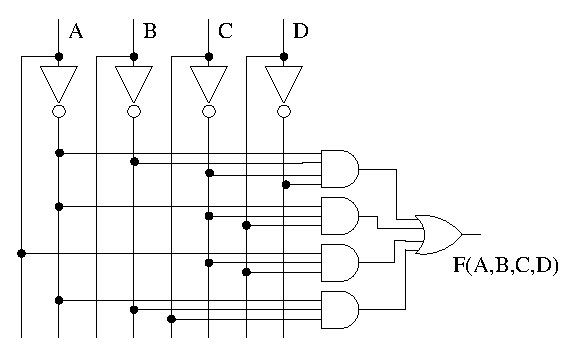
\includegraphics{Prob3-3}}
\label{fig:Hw3}
\end{figure}

\begin{onlysolution}  \textbf{Solution} \itshape{
From the circuit we have:
F(A,B,C,D) = A'B'C'D' + A'C'D + AC'D + A'B'C
$$ \begin{array} {c||c|c|c|c}
       AB \bs CD & 00 & 01 & 11 & 10 \\ \hline \hline
       00        & 1  & 1  & 1  & 1  \\ \hline
       01        &    & 1  &    &    \\ \hline
       11        &    & 1  &    &    \\ \hline
       10        &    & 1  &    &    \\
\end{array} $$ 
From this it follows that 
F(A,B,C,D) =  A'B' + C'D
} \end{onlysolution} 

\item  \textbf{ (8 pts.)} Design a digital system with four bits of inputs 
$I_3 I_2 I_1 I_0$ and two bits of outputs $O_1 O_0$.  At least one
of the inputs is always equal to 1.  The output encodes the 
index of the most significant 1 in the input.
For example, if $I_3 I_2 I_1 I_0 = 0101$, then the index
of the most significant 1 is 2, hence $O_1 O_0 = 10$.  Submit:
\begin{itemize}
\item The truth table.

\begin{onlysolution}  \textbf{Solution} \itshape{
	\begin{tabular}{l|l|l|l||l|l}
	$I_3$ & $I_2$ & $I_1$ & $I_0$ & $O_1$ & $O_0$ \\ \hline
	0 & 0 & 0 & 0 &  x & x \\ \hline
	0 & 0 & 0 & 1 &  0 & 0 \\ \hline
	0 & 0 & 1 & 0 &  0 & 1 \\ \hline
	0 & 0 & 1 & 1 &  0 & 1 \\ \hline
	0 & 1 & 0 & 0 &  1 & 0 \\ \hline
	0 & 1 & 0 & 1 &  1 & 0 \\ \hline
	0 & 1 & 1 & 0 &  1 & 0 \\ \hline
	0 & 1 & 1 & 1 &  1 & 0 \\ \hline
	1 & 0 & 0 & 0 &  1 & 1 \\ \hline
	1 & 0 & 0 & 1 &  1 & 1 \\ \hline
	1 & 0 & 1 & 0 &  1 & 1 \\ \hline
	1 & 0 & 1 & 1 &  1 & 1 \\ \hline
	1 & 1 & 0 & 0 &  1 & 1 \\ \hline
	1 & 1 & 0 & 1 &  1 & 1 \\ \hline
	1 & 1 & 1 & 0 &  1 & 1 \\ \hline
	1 & 1 & 1 & 1 &  1 & 1 \\ 
	\end{tabular}
} \end{onlysolution} 
\item \SOPmin expression for $O_1$ and $O_0$.

\begin{onlysolution}  \textbf{Solution} \itshape{
\begin{tabular}{ll}
$ \begin{array} {c||c|c|c|c}
 I3 I2 \bs I1 I0 & 00 & 01 & 11 & 10 \\ \hline \hline
       00        & x  &    &    &    \\ \hline
       01        & 1  & 1  & 1  & 1  \\ \hline
       11        & 1  & 1  & 1  & 1  \\ \hline
       10        & 1  & 1  & 1  & 1  \\
\end{array} $ & 
$ \begin{array} {c||c|c|c|c}
 I3 I2 \bs I1 I0 & 00 & 01 & 11 & 10 \\ \hline \hline
       00        & x  &    & 1  & 1  \\ \hline
       01        &    &    &    &    \\ \hline
       11        & 1  & 1  & 1  & 1  \\ \hline
       10        & 1  & 1  & 1  & 1  \\
\end{array} $ \\
$O_1 = I_3 + I_2$ & $O_0=I_3 + I_2'I_1$ \\
\end{tabular}
} \end{onlysolution} 
\end{itemize}

\item \textbf{ (8 pts.)}
Design a 4-input $a_1 a_0 b_1 b_0$, 4 -output $O_3 O_2 O_1 O_0$
digital system.  $A=a_1 a_0$ and $B=b_1 b_0$ represent 2-bit binary
numbers.  The output should be the product (multiplication) of the inputs, 
that is $O = A*B$.  In addition to determining the output, determine the
number of bits of output. Submit:
\begin{itemize}
\item Truth tables.

\begin{onlysolution}  \textbf{Solution} \itshape{
\begin{tabular}{l|l|l|l||l|l|l|l}
$a_1$ & $a_0$ & $b_1$ & $b_0$ & $O_3$ & $O_2$ & $O_1$ & $O_0$ \\ \hline
0&0&0&0 &0&0&0&0 \\ \hline
0&0&0&1 &0&0&0&0 \\ \hline
0&0&1&0 &0&0&0&0 \\ \hline
0&0&1&1 &0&0&0&0 \\ \hline
0&1&0&0 &0&0&0&0 \\ \hline
0&1&0&1 &0&0&0&1 \\ \hline
0&1&1&0 &0&0&1&0 \\ \hline
0&1&1&1 &0&0&1&1 \\ \hline
1&0&0&0 &0&0&0&0 \\ \hline
1&0&0&1 &0&0&1&0 \\ \hline
1&0&1&0 &0&1&0&0 \\ \hline
1&0&1&1 &0&1&1&0 \\ \hline
1&1&0&0 &0&0&0&0 \\ \hline
1&1&0&1 &0&0&1&1 \\ \hline
1&1&1&0 &0&1&1&0 \\ \hline
1&1&1&1 &1&0&0&1 \\
\end{tabular}
} \end{onlysolution} 

\item Minimal SOP expression for the outputs.

\begin{onlysolution}  \textbf{Solution} \itshape{
\begin{tabular}{ll}
$\begin{array} {c||c|c|c|c}
 a1 a0 \bs b1 b0 & 00 & 01 & 11 & 10 \\ \hline \hline
       00        &    &    &    &    \\ \hline
       01        &    &    &    &    \\ \hline
       11        &    &    & 1  &    \\ \hline
       10        &    &    &    &    \\
\end{array}$ &
$\begin{array} {c||c|c|c|c}
 a1 a0 \bs b1 b0 & 00 & 01 & 11 & 10 \\ \hline \hline
       00        &    &    &    &    \\ \hline
       01        &    &    &    &    \\ \hline
       11        &    &    &    & 1  \\ \hline
       10        &    &    & 1  & 1  \\
\end{array} $ \\
$O_3 = a_1a_0b_1b_0$ & $O_2 = a_1a_0'b_1 + a_1b_1b_0'$\\
\end{tabular}
} \end{onlysolution} 


\begin{onlysolution}  \textbf{Solution} \itshape{
\begin{tabular}{ll}
$\begin{array} {c||c|c|c|c}
 a1 a0 \bs b1 b0 & 00 & 01 & 11 & 10 \\ \hline \hline
       00        &    &    &    &    \\ \hline
       01        &    &    & 1  & 1  \\ \hline
       11        &    & 1  &    & 1  \\ \hline
       10        &    & 1  & 1  &    \\
\end{array}$ &
$\begin{array} {c||c|c|c|c}
 a1 a0 \bs b1 b0 & 00 & 01 & 11 & 10 \\ \hline \hline
       00        &    &    &    &    \\ \hline
       01        &    & 1  & 1  &    \\ \hline
       11        &    & 1  & 1  &    \\ \hline
       10        &    &    &    &    \\
\end{array}$ \\
$O_1 = a_1b_1'b_0 + a_1a_0'b_0 + a_1'a_0b_1+a_0b_1b_0'$ & $O_0 = a_0b_0$ \\
\end{tabular}
} \end{onlysolution} 

\end{itemize}

\item  \textbf{ (8 pts.)}
Design a 4-bit Gray-code to binary converter.  A 4-bit gray-code is a 
sequence of 4-bit values where successive values differ by a single
bit.  For this problem use the sequence: 0000, 0001, 0011, 0010, 
0110, 0111, 0101, 0100, 1100, 1101, 1111, 1110, 1010, 1011, 1001, 
1000.  The index of the 4-bit gray code is its binary value.  For
example, the 4-bit gray code 0111 is at index 5, therefore when
presented with 0111 on its input, the converter should output 0101.
Submit:
\begin{itemize}
\item A truth table for the converter.

\begin{onlysolution}  \textbf{Solution} \itshape{
\begin{tabular}{l|l|l|l||l|l|l|l}
$a_3$ & $a_2$ & $a_1$ & $a_0$ & $f_3$ & $f_2$ & $f_1$ & $f_0$ \\ \hline
0&0&0&0 &0&0&0&0 \\ \hline
0&0&0&1 &0&0&0&1 \\ \hline
0&0&1&0 &0&0&1&1 \\ \hline
0&0&1&1 &0&0&1&0 \\ \hline
0&1&0&0 &0&1&1&0 \\ \hline
0&1&0&1 &0&1&1&1 \\ \hline
0&1&1&0 &0&1&0&1 \\ \hline
0&1&1&1 &0&1&0&0 \\ \hline
1&0&0&0 &1&1&0&0 \\ \hline
1&0&0&1 &1&1&0&1 \\ \hline
1&0&1&0 &1&1&1&1 \\ \hline
1&0&1&1 &1&1&1&0 \\ \hline
1&1&0&0 &1&0&1&0 \\ \hline
1&1&0&1 &1&0&1&1 \\ \hline
1&1&1&0 &1&0&0&1 \\ \hline
1&1&1&1 &1&0&0&0 \\ 
\end{tabular}
} \end{onlysolution} 

\item Four k-maps for the converter.

\begin{onlysolution}  \textbf{Solution} \itshape{
\begin{tabular}{ll}
$\begin{array} {c||c|c|c|c}
 a3 a2 \bs a1 a0 & 00 & 01 & 11 & 10 \\ \hline \hline
       00        &    &    &    &    \\ \hline
       01        &    &    &    &    \\ \hline
       11        & 1  & 1  & 1  & 1  \\ \hline
       10        & 1  & 1  & 1  & 1  \\
\end{array}$ &
$\begin{array} {c||c|c|c|c}
 a3 a2 \bs a1 a0 & 00 & 01 & 11 & 10 \\ \hline \hline
       00        &    &    &    &    \\ \hline
       01        & 1  & 1  & 1  & 1  \\ \hline
       11        &    &    &    &    \\ \hline
       10        & 1  & 1  & 1  & 1  \\
\end{array} $ \\
$f_3 = a_3$ & $f_2 = a_3a_2'+a_3'a_2$\\
\end{tabular}
} \end{onlysolution} 


\begin{onlysolution}  \textbf{Solution} \itshape{
\begin{tabular}{ll}
$\begin{array} {c||c|c|c|c}
 a3 a2 \bs a1 a0 & 00 & 01 & 11 & 10 \\ \hline \hline
       00        &    &    & 1  & 1  \\ \hline
       01        & 1  & 1  &    &    \\ \hline
       11        & 1  & 1  &    &    \\ \hline
       10        &    &    & 1  & 1  \\
\end{array}$ &
$\begin{array} {c||c|c|c|c}
 a3 a2 \bs a1 a0 & 00 & 01 & 11 & 10 \\ \hline \hline
       00        &    & 1  &    & 1  \\ \hline
       01        &    & 1  &    & 1  \\ \hline
       11        &    & 1  &    & 1  \\ \hline
       10        &    & 1  &    & 1  \\
\end{array}$ \\
$f_1 = a_2a_1'+a_2'a_1$ & $f_0 = a_1'a_0+a_1a_0'$ \\
\end{tabular}
} \end{onlysolution} 

\item \SOPmin expression for the outputs, no product sharing please
(use the \verb+-Dso+ command line option).
\item Espresso file for the converter
\item Espresso output in PLA format
\item Compare the number of gates required in your solution
versus the number of gates required by Espresso.
\end{itemize}

\item \textbf{ (4 pts. each)} Determine \SOPmin expression for:
\begin{enumerate}
\item $F(A,B,C)=\sum m(0,1,3,4,5)$

\begin{onlysolution}  \textbf{Solution} \itshape{
$\begin{array} {c||c|c|c|c}
   A   \bs B C  & 00 & 01 & 11 & 10 \\ \hline \hline
       0        &  1 & 1  & 1  &    \\ \hline
       1        &  1 & 1  &    &    \\ 
\end{array}$ \\
F(A,B,C)= B'+A'C
} \end{onlysolution} 
\item $F(A,B,C,D)=\sum m(1,5,6,7,11,12,13,15)$

\begin{onlysolution}  \textbf{Solution} \itshape{
$\begin{array} {c||c|c|c|c}
   A B \bs C D   & 00 & 01 & 11 & 10 \\ \hline \hline
       00        &    & 1  &    &    \\ \hline
       01        &    & 1  & 1  & 1  \\ \hline
       11        & 1  & 1  & 1  &    \\ \hline
       10        &    &    & 1  &    \\
\end{array}$  \\
F(A,B,C)= ABC'+A'C'D+ACD+A'BC
} \end{onlysolution} 
\item $F(A,B,C,D)=\sum m(0,2,5,6,8,11,12,13,14,15)$

\begin{onlysolution}  \textbf{Solution} \itshape{
$\begin{array} {c||c|c|c|c}
   A B \bs C D   & 00 & 01 & 11 & 10 \\ \hline \hline
       00        & 1  &    &    & 1  \\ \hline
       01        &    & 1  &    & 1  \\ \hline
       11        & 1  & 1  & 1  & 1  \\ \hline
       10        & 1  &    & 1  &    \\
\end{array}$  \\
F(A,B,C,D) =  AB + BC'D + ACD + B'C'D' + A'CD'
} \end{onlysolution} 
\item $F(A,B,C,D,E)=\sum m(0,8,9,10,13,15,22,26,29,30,31)$

\begin{onlysolution}  \textbf{Solution} \itshape{
\begin{tabular}{cc}
$\begin{array} {c||c|c|c|c}
   B C \bs D E   & 00 & 01 & 11 & 10 \\ \hline \hline
       00        & 1  &    &    &    \\ \hline
       01        &    &    &    &    \\ \hline
       11        &    & 1  & 1  &    \\ \hline
       10        & 1  & 1  &    & 1  \\
\end{array}$ &
$\begin{array} {c||c|c|c|c}
   B C \bs D E   & 00 & 01 & 11 & 10 \\ \hline \hline
       00        &    &    &    &    \\ \hline
       01        &    &    &    & 1  \\ \hline
       11        &    & 1  & 1  & 1  \\ \hline
       10        &    &    &    & 1  \\
\end{array}$ \\
A=0 & A=1 \\
\end{tabular} \\
F(A,B,C,D,E) = BCE + A'C'D'E' + BC'DE + ACDE' + A'BD'E or \\
F(A,B,C,D,E) = BCE + A'C'D'E' + BC'DE + ACDE' + A'BC'D'
} \end{onlysolution} 

\item $F(A,B,C,D,E)=\sum m(0,2,4,5,7,10,13,15,18,21,24,26,28,29)$

\begin{onlysolution}  \textbf{Solution} \itshape{
\begin{tabular}{cc}
$\begin{array} {c||c|c|c|c}
   B C \bs D E   & 00 & 01 & 11 & 10 \\ \hline \hline
       00        & 1  &    &    & 1  \\ \hline
       01        & 1  & 1  & 1  &    \\ \hline
       11        &    & 1  & 1  &    \\ \hline
       10        &    &    &    & 1  \\
\end{array}$ &
$\begin{array} {c||c|c|c|c}
   B C \bs D E   & 00 & 01 & 11 & 10 \\ \hline \hline
       00        &    &    &    & 1  \\ \hline
       01        &    & 1  &    &    \\ \hline
       11        & 1  & 1  &    &    \\ \hline
       10        & 1  &    &    & 1  \\
\end{array}$ \\
A=0 & A=1 \\
\end{tabular} \\
F(A,B,C,D,E) = A'B'D'E' + CD'E+C'DE'+ABD'E'+A'CE
} \end{onlysolution} 

\end{enumerate}

\item \textbf{ (4 pts. each)} Determine \SOPmin expression for:
\begin{enumerate}
\item $F(A,B,C,D)=\sum m(4,7,9,12,13,15)+\sum d(0,1,2,3,10,14)$

\begin{onlysolution}  \textbf{Solution} \itshape{
$\begin{array} {c||c|c|c|c}
   A B \bs C D   & 00 & 01 & 11 & 10 \\ \hline \hline
       00        & x  & x  & x  &    \\ \hline
       01        & 1  &    & 1  &    \\ \hline
       11        & 1  & 1  & 1  & x  \\ \hline
       10        &    & 1  &    & x  \\
\end{array}$  \\
F(A,B,C,D) = BC'D'+AC'D+BCD
} \end{onlysolution} 

\item $F(A,B,C,D)=\sum m(0,1,5,7,10,14,15)+\sum d(2,8)$

\begin{onlysolution}  \textbf{Solution} \itshape{
$\begin{array} {c||c|c|c|c}
   A B \bs C D   & 00 & 01 & 11 & 10 \\ \hline \hline
       00        & 1  & 1  &    & x  \\ \hline
       01        &    & 1  & 1  &    \\ \hline
       11        &    &    & 1  & 1  \\ \hline
       10        & x  &    &    & 1  \\
\end{array}$ \\
F(A,B,C,D) = B'D'+A'C'D+BCD+ABC
} \end{onlysolution} 
\item $F(A,B,C,D)=\sum m(0,1,3,4,15)+\sum d(10,12)$

\begin{onlysolution}  \textbf{Solution} \itshape{

$\begin{array} {c||c|c|c|c}
   A B \bs C D   & 00 & 01 & 11 & 10 \\ \hline \hline
       00        & 1  & 1  & 1  &    \\ \hline
       01        & 1  &    &    &    \\ \hline
       11        & x  &    & 1  &    \\ \hline
       10        &    &    &    & x  \\
\end{array}$ \\
F(A,B,C,D)=ABCD+A'C'D'+A'B'D
} \end{onlysolution} 
\item $F(A,B,C,D,E)=\sum m(2,3,5,7,11,13,17,19,29,31)+\sum d(1,4,9,16,25)$

\begin{onlysolution}  \textbf{Solution} \itshape{

\begin{tabular}{cc}
$\begin{array} {c||c|c|c|c}
   B C \bs D E   & 00 & 01 & 11 & 10 \\ \hline \hline
       00        &    & x  & 1  & 1  \\ \hline
       01        & x  & 1  & 1  &    \\ \hline
       11        &    & 1  &    &    \\ \hline
       10        &    & x  & 1  &    \\
\end{array}$ &
$\begin{array} {c||c|c|c|c}
   B C \bs D E   & 00 & 01 & 11 & 10 \\ \hline \hline
       00        & x  & 1  & 1  &    \\ \hline
       01        &    &    &    &    \\ \hline
       11        &    & 1  & 1  &    \\ \hline
       10        &    & x  &    &    \\
\end{array}$ \\
A=0 & A=1 \\
\end{tabular} \\
F(A,B,C,D,E)=A'D'E+A'C'E+A'B'C'D+B'C'E+ABCE +A'B'E
} \end{onlysolution} 

\item $F(A,B,C,D,E)=\sum m(2,3,6,10,12,13,14,18,25,26,28,29)+\sum d(11,27)$

\begin{onlysolution}  \textbf{Solution} \itshape{

\begin{tabular}{cc}
$\begin{array} {c||c|c|c|c}
   B C \bs D E   & 00 & 01 & 11 & 10 \\ \hline \hline
       00        &    &    & 1  & 1  \\ \hline
       01        &    &    &    & 1  \\ \hline
       11        & 1  & 1  &    & 1  \\ \hline
       10        &    &    & x  & 1  \\
\end{array}$ &
$\begin{array} {c||c|c|c|c}
   B C \bs D E   & 00 & 01 & 11 & 10 \\ \hline \hline
       00        &    &    &    & 1  \\ \hline
       01        &    &    &    &    \\ \hline
       11        & 1  & 1  &    &    \\ \hline
       10        &    & 1  & x  & 1  \\
\end{array}$ \\
A=0 & A=1 \\
\end{tabular} \\
F(A,B,C,D,E)=A'C'D+C'DE'+A'DE' +BCD' + ABC'E 
} \end{onlysolution} 

\end{enumerate}

\item \textbf{ (8 pts. each)} Determine \SOPmin and \POSmin expressions for:
\begin{enumerate}
\item  $F(A,B,C,D) = \sum m(0,1,2,5,8,10,13,15)$

\begin{onlysolution}  \textbf{Solution} \itshape{

\begin{tabular}{cc}
$\begin{array} {c||c|c|c|c}
   A B \bs C D   & 00 & 01 & 11 & 10 \\ \hline \hline
       00        & 1  & 1  &    & 1  \\ \hline
       01        &    & 1  &    &    \\ \hline
       11        &    & 1  & 1  &    \\ \hline
       10        & 1  &    &    & 1  \\
\end{array}$ &
$\begin{array} {c||c|c|c|c}
   A B \bs C D   & 00 & 01 & 11 & 10 \\ \hline \hline
       00        &    &    & 1  &    \\ \hline
       01        & 1  &    & 1  & 1  \\ \hline
       11        & 1  &    &    & 1  \\ \hline
       10        &    & 1  & 1  &    \\
\end{array}$ \\
F  & F' \\
\end{tabular} \\
\SOPmin F(A,B,C,D) =  B'D'+A'C'D+ABD\\
\POSmin F(A,B,C,D) =  (B'+D)(A+C'+D')(A'+B+D')
} \end{onlysolution} 

\item  $F(A,B,C,D) = \prod M(0,4,6,10,11,12)$

\begin{onlysolution}  \textbf{Solution} \itshape{

\begin{tabular}{cc}
$\begin{array} {c||c|c|c|c}
   A B \bs C D   & 00 & 01 & 11 & 10 \\ \hline \hline
       00        &    & 1  & 1  & 1  \\ \hline
       01        &    & 1  & 1  &    \\ \hline
       11        &    & 1  & 1  & 1  \\ \hline
       10        & 1  & 1  &    &    \\
\end{array}$ &
$\begin{array} {c||c|c|c|c}
   A B \bs C D   & 00 & 01 & 11 & 10 \\ \hline \hline
       00        & 1  &    &    &    \\ \hline
       01        & 1  &    &    & 1  \\ \hline
       11        & 1  &    &    &    \\ \hline
       10        &    &    & 1  & 1  \\
\end{array}$ \\
F  & F' \\
\end{tabular} \\
\SOPmin F(A,B,C,D) = AB'C'+A'B'C+ABC+C'D+A'D  or \\
\SOPmin F(A,B,C,D) = AB'C'+A'B'C+ABC+C'D+BD  or \\
\SOPmin F(A,B,C,D) = AB'C'+A'B'C+ABC+A'D+BD \\
\POSmin F(A,B,C,D) =  (A+C+D)(B'+C+D)(A+B'+D)(A'+B+C')
} \end{onlysolution} 
\item  $F(A,B,C,D) = \sum m(0,5,7,10,11,14) + \sum d(3,12,15)$

\begin{onlysolution}  \textbf{Solution} \itshape{

\begin{tabular}{cc}
$\begin{array} {c||c|c|c|c}
   A B \bs C D   & 00 & 01 & 11 & 10 \\ \hline \hline
       00        & 1  &    & x  &    \\ \hline
       01        &    & 1  & 1  &    \\ \hline
       11        & x  &    & x  & 1  \\ \hline
       10        &    &    & 1  & 1  \\
\end{array}$ &
$\begin{array} {c||c|c|c|c}
   A B \bs C D   & 00 & 01 & 11 & 10 \\ \hline \hline
       00        &    & 1  & x  & 1  \\ \hline
       01        & 1  &    &    & 1  \\ \hline
       11        & x  & 1  & x  &    \\ \hline
       10        & 1  & 1  &    &    \\
\end{array}$ \\
F  & F' \\
\end{tabular} \\
\SOPmin F(A,B,C,D) =  A'B'C'D'+A'BD+AC\\
\POSmin F(A,B,C,D) =  (A'+C)(A+C'+D)(A+B+D')(B'+C+D) or \\ 
\POSmin F(A,B,C,D) =  (A'+C)(A+C'+D)(B+C+D')(B'+C+D) or \\ 
\POSmin F(A,B,C,D) =  (A'+C)(A+C'+D)(A+B+D')(A+B'+D) or \\ 
\POSmin F(A,B,C,D) =  (A'+C)(A+C'+D)(B+C+D')(A+B'+D)  \\ 
} \end{onlysolution} 
\item  $F(A,B,C,D) = \prod M(2,6,7,9,15) * \prod d(4,12,13) $

\begin{onlysolution}  \textbf{Solution} \itshape{

\begin{tabular}{cc}
$\begin{array} {c||c|c|c|c}
   A B \bs C D   & 00 & 01 & 11 & 10 \\ \hline \hline
       00        & 1  & 1  & 1  &    \\ \hline
       01        & x  & 1  &    &    \\ \hline
       11        & x  & x  &    & 1  \\ \hline
       10        & 1  &    & 1  & 1  \\
\end{array}$ &
$\begin{array} {c||c|c|c|c}
   A B \bs C D   & 00 & 01 & 11 & 10 \\ \hline \hline
       00        &    &    &    & 1  \\ \hline
       01        & x  &    & 1  & 1  \\ \hline
       11        & x  & x  & 1  &    \\ \hline
       10        &    & 1  &    &    \\
\end{array}$ \\
F  & F' \\
\end{tabular} \\
\SOPmin F(A,B,C,D) =  A'C'+AD'+A'CD\\
\POSmin F(A,B,C,D) =  (A+C'+D)(B'+C'+D')(A'+C+D')
} \end{onlysolution} 
\item  $F(W,X,Y,Z) = WX'Z' + X'YZ + W'Y'Z + XYZ + WXY'$

\begin{onlysolution}  \textbf{Solution} \itshape{
\begin{tabular}{cc}
$\begin{array} {c||c|c|c|c}
   W X \bs Y Z   & 00 & 01 & 11 & 10 \\ \hline \hline
       00        &    & 1  & 1  &    \\ \hline
       01        &    & 1  & 1  &    \\ \hline
       11        & 1  & 1  & 1  &    \\ \hline
       10        & 1  &    & 1  & 1  \\
\end{array}$ &
$\begin{array} {c||c|c|c|c}
   W X \bs Y Z   & 00 & 01 & 11 & 10 \\ \hline \hline
       00        & 1  &    &    & 1  \\ \hline
       01        & 1  &    &    & 1  \\ \hline
       11        &    &    &    & 1  \\ \hline
       10        &    & 1  &    &    \\
\end{array}$ \\
F  & F' \\
\end{tabular} \\
\SOPmin F(W,X,Y,Z) =  W'Z+XZ+WY'Z'+WX'Y\\
\POSmin F(W,X,Y,Z) = (W+Z)(X'+Y'+Z)(W'+X+Y+Z')
} \end{onlysolution} 

\item  $F(W,X,Y,Z) = (W + X'+Y')(W'+Z')(W+Y')$

\begin{onlysolution}  \textbf{Solution} \itshape{

We have that $F'(W,X,Y,Z) = W'XY+ WZ+ W'Y$

\begin{tabular}{cc}
$\begin{array} {c||c|c|c|c}
   W X \bs Y Z   & 00 & 01 & 11 & 10 \\ \hline \hline
       00        &    &    & 1  & 1  \\ \hline
       01        &    &    & 1  & 1  \\ \hline
       11        &    & 1  & 1  &    \\ \hline
       10        &    & 1  & 1  &    \\
\end{array}$ &
$\begin{array} {c||c|c|c|c}
   W X \bs Y Z   & 00 & 01 & 11 & 10 \\ \hline \hline
       00        & 1  & 1  &    &    \\ \hline
       01        & 1  & 1  &    &    \\ \hline
       11        & 1  &    &    & 1  \\ \hline
       10        & 1  &    &    & 1  \\
\end{array}$ \\
F'  & F \\
\end{tabular} \\
\SOPmin F(W,X,Y,Z) =  W'Y'+WZ'\\
\POSmin F(W,X,Y,Z) = (W'+Z')(W+Y')
} \end{onlysolution} 
\end{enumerate}
Hint, the negation of a ``Don't care" is a ``Don't care".

\item \textbf{ (3 pts.)} While grading homework for a digital design class 
the following question/answer pair is encountered.  What is 
the problem with the answer given?

\begin{tabular}{l}
Question: Generate the \POSmin expression for $F(A,B,C) = \sum m(2,3,4,5)$ \\
Answer: $F(A,B,C) = (A+B')(A'+B)$ \\
\end{tabular}

\item \textbf{ (6 pts.)} Determine the \SOPmin realization of the following
function.

\begin{tabular}{c|c|c|c||c}
A & B & C & D & F(A,B,C,D) \\ \hline
x & 1 & 1 & x & 0 \\ \hline
0 & x & 0 & 1 & 0 \\ \hline
x & x & 0 & 0 & x \\ \hline
x & 0 & 1 & x & 1 \\ \hline
1 & x & 0 & 1 & 1 \\ 
\end{tabular}


\begin{onlysolution}  \textbf{Solution} \itshape{
$\begin{array} {c||c|c|c|c}
   A B \bs B C   & 00 & 01 & 11 & 10 \\ \hline \hline
       00        & x  & 0  & 1  & 1  \\ \hline
       01        & x  & 0  & 0  & 0  \\ \hline
       11        & x  & 1  & 0  & 0  \\ \hline
       10        & x  & 1  & 1  & 1  \\
\end{array}$  \\
F(A,B,C) = AC'+B'C
} \end{onlysolution} 

\item \textbf{ (6 pts.)} What is the worst function \SOPmin of 3 variable 
that can be created?  That is, define a function whose minimal SOP form 
has the largest possible number of product terms.  What is the largest 
number of product terms that a 4-variable \SOPmin expression can 
have?  How about $N$ variables?

\begin{onlysolution}  \textbf{Solution} \itshape{
The worst function of three variable is shown in the Kmap below:

$\begin{array} {c||c|c|c|c}
   A \bs B C   & 00 & 01 & 11 & 10 \\ \hline \hline
      0        & 1  &    & 1  &    \\ \hline
      1        &    & 1  &    & 1  \\ 
\end{array}$

This function requires four product terms.  Any additional minterm added to 
this Kmap would create a grouping with neighboring minterms, perhaps not 
decreasing the
the number of product terms, but certainly making the product terms simpler.
Its important to note that this configuration looks like a checkerboard.
The worst function of four variables looks like:

$\begin{array} {c||c|c|c|c}
   A B \bs B C   & 00 & 01 & 11 & 10 \\ \hline \hline
       00        & 1  &    & 1  &    \\ \hline
       01        &    & 1  &    & 1  \\ \hline
       11        & 1  &    & 1  &    \\ \hline
       10        &    & 1  &    & 1  \\
\end{array}$

This function requires 8 product terms, each containing every variable.  Boy that's
one bad realization.  In a general, the worst realization of an $N$ variable function 
requires $2^{N-1}$ product terms.  This is because the checkerboard configuration can
be applied to any Kmap, with half of the cells containing 1's.  Since a function with
$N$ variables has $2^{N}$ cells, then 1/2 of these cells works out to $2^{N-1}$.
} \end{onlysolution}  


\item \textbf{ (16 pts.)} Sometimes a logic circuit needs to output 
a logic 0 in order to produce some behavior.  For example, an LED can be
attached to a digital circuit output so that it lights up when the circuit
outputs a 0.  This response is called an active low output; the output
device is \textit{ active} then the digital output is \textit{ low}.
                                                                                
Build a digital circuit that takes as input two 2-bit numbers,
A and B.  The circuit has three outputs which drive three
LEDs labeled G, L, and E.
The G LED should be illuminated when A$>$B.
The L LED should be illuminated when A$<$B.
The E LED should be illuminated when A=B.
The LEDs are illuminated when the circuit outputs a 0, otherwise
they are turned off.
                                                                                
Determine \SOPmin expression for the G, L and E outputs.
Determine \POSmin expression for the G, L and E outputs.
                                                                                


\end{enumerate}
